\documentclass[aspectratio=169,10pt]{beamer}
\usepackage[T1]{fontenc}
\usepackage[utf8]{inputenc}
\usepackage{lmodern}
\usepackage{amsmath,amssymb,bm,mathtools}
\usepackage{xcolor}
\usepackage{tikz}
\usetikzlibrary{arrows.meta,positioning}
\setbeamersize{text margin left=7mm,text margin right=7mm}
\setbeamertemplate{navigation symbols}{}
\setbeamertemplate{footline}{}
\setbeamerfont{frametitle}{series=\bfseries,size=\Large}
\definecolor{radblue}{RGB}{18,78,155}
\definecolor{radgreen}{RGB}{25,125,65}
\definecolor{radorange}{RGB}{225,105,20}
\definecolor{radred}{RGB}{185,35,30}
\definecolor{lightblue}{RGB}{235,243,255}
\definecolor{lightgreen}{RGB}{237,249,241}
\definecolor{lightorange}{RGB}{255,244,232}
\definecolor{lightred}{RGB}{255,240,238}
\definecolor{lightgray}{RGB}{248,248,248}
\newcommand{\qrad}{\dot{q}_{\mathrm{rad}}}
\newcommand{\Mfull}{\mathcal{M}_{\mathrm{full}}}
\newcommand{\Mred}{\mathcal{M}_{\mathrm{red}}}
\newcommand{\ydev}{y_{\mathrm{device}}}
\newcommand{\J}{\bm{J}}

\begin{document}

\begin{frame}{Module 8: Reduced-fidelity modeling strategy}
\footnotesize
\vspace{-2mm}
\begin{center}
\fbox{\parbox{0.91\textwidth}{\centering
Approximate the full model by a cheaper model while preserving the device-level response:
\[
\Mfull(\bm{x}_{\mathrm{full}})=\ydev,\qquad
\Mred(\bm{x}_{\mathrm{red}})=\widehat{\ydev},\qquad
\varepsilon_{\mathrm{red}}=\frac{\|\widehat{\ydev}-\ydev\|}{\|\ydev\|}\leq\varepsilon_{\mathrm{tol}}.
\]
}}
\end{center}
\vspace{1.5mm}
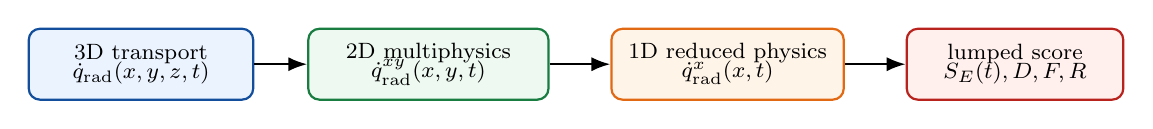
\begin{tikzpicture}[x=1cm,y=1cm,every node/.style={font=\footnotesize},
box/.style={rounded corners,draw,thick,align=center,minimum height=0.9cm},
arr/.style={-{Latex[length=2.4mm]},thick}]
\node[box,fill=lightblue,draw=radblue,minimum width=2.85cm] (A) at (0,0) {3D transport\\[-1mm]$\qrad(x,y,z,t)$};
\node[box,fill=lightgreen,draw=radgreen,minimum width=3.05cm] (B) at (3.65,0) {2D multiphysics\\[-1mm]$\qrad^{xy}(x,y,t)$};
\node[box,fill=lightorange,draw=radorange,minimum width=2.95cm] (C) at (7.45,0) {1D reduced physics\\[-1mm]$\qrad^x(x,t)$};
\node[box,fill=lightred,draw=radred,minimum width=2.75cm] (D) at (11.1,0) {lumped score\\[-1mm]$S_E(t),D,F,R$};
\draw[arr] (A) -- (B);
\draw[arr] (B) -- (C);
\draw[arr] (C) -- (D);
\end{tikzpicture}
\vspace{1mm}
\[
\qrad^{xy}(x,y,t)=\frac{1}{L_z}\int \qrad(x,y,z,t)\,dz,
\quad
\qrad^x(x,t)=\frac{1}{L_y}\int \qrad^{xy}(x,y,t)\,dy,
\quad
S_E(t)=\int_V\qrad\,dV.
\]
\vspace{1mm}
\begin{columns}[T,totalwidth=\textwidth]
\begin{column}{0.55\textwidth}
\textbf{Dominant-path reduction}
\[
\qrad \rightarrow C_j \rightarrow \rho,\phi,T \rightarrow n,p,\J \rightarrow \ydev
\]
\[
\Downarrow\; \text{select the few paths that control }\ydev
\]
\[
\qrad \rightarrow C_{\mathrm{eff}} \rightarrow \phi_{\mathrm{eff}},\J_{\mathrm{eff}} \rightarrow \widehat{\ydev}
\]
\end{column}
\begin{column}{0.41\textwidth}
\textbf{Model-selection principle}
\vspace{1mm}

Keep high-impact physics. Reduce or bypass physics that is expensive but weakly coupled to the selected device metric.
\end{column}
\end{columns}
\end{frame}

\begin{frame}{Module 8: Impact-cost importance scoring}
\footnotesize
\vspace{-2mm}
\begin{columns}[T,totalwidth=\textwidth]
\begin{column}{0.48\textwidth}
\textbf{1. Estimate impact}\vspace{-1mm}
\[
I_m=\frac{\|\ydev^{\mathrm{base}}-\ydev^{(-m)}\|}{\|\ydev^{\mathrm{base}}\|},
\qquad
I_m \approx \left\|\frac{\partial\ydev}{\partial\theta_m}\Delta\theta_m\right\|.
\]
\begin{itemize}\setlength\itemsep{0mm}
\item Ablation: remove or simplify part $m$.
\item Sensitivity: perturb parameter or source $\theta_m$.
\end{itemize}
\vspace{1mm}
\textbf{2. Estimate computational cost}\vspace{-1mm}
\[
C_m \approx T_mN_{\mathrm{calls}},
\qquad
C_m\sim N_{\mathrm{dof}}^{\alpha}N_tN_{\mathrm{iter}}.
\]
\begin{itemize}\setlength\itemsep{0mm}
\item Use timing logs when available.
\item Use complexity estimates before implementation.
\end{itemize}
\end{column}
\begin{column}{0.48\textwidth}
\textbf{3. Normalize and rank}\vspace{-1mm}
\[
\widetilde I_m=\frac{I_m}{\max_k I_k},
\qquad
\widetilde C_m=\frac{C_m}{\max_k C_k},
\qquad
\boxed{\Pi_m=\frac{\widetilde I_m}{\widetilde C_m+\varepsilon_0}}.
\]
\vspace{1mm}
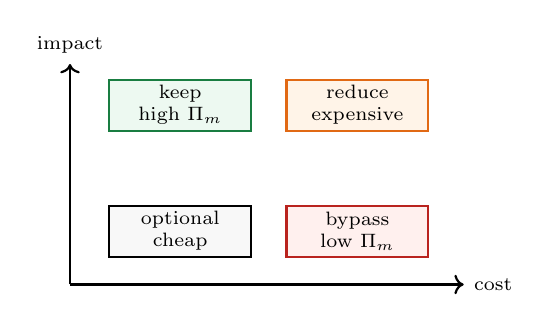
\begin{tikzpicture}[x=1cm,y=1cm,every node/.style={font=\scriptsize}]
\draw[->,thick] (0,0) -- (5.0,0) node[right]{cost};
\draw[->,thick] (0,0) -- (0,2.8) node[above]{impact};
\draw[fill=lightgreen,draw=radgreen,thick] (0.50,1.95) rectangle (2.30,2.60);
\node[align=center] at (1.40,2.28) {keep\\high $\Pi_m$};
\draw[fill=lightorange,draw=radorange,thick] (2.75,1.95) rectangle (4.55,2.60);
\node[align=center] at (3.65,2.28) {reduce\\expensive};
\draw[fill=lightgray,draw=black,thick] (0.50,0.35) rectangle (2.30,1.00);
\node[align=center] at (1.40,0.68) {optional\\cheap};
\draw[fill=lightred,draw=radred,thick] (2.75,0.35) rectangle (4.55,1.00);
\node[align=center] at (3.65,0.68) {bypass\\low $\Pi_m$};
\end{tikzpicture}
\vspace{1mm}

\textbf{Decision rule:} retain high-impact terms; reduce expensive but important terms; bypass low-impact expensive terms.
\end{column}
\end{columns}
\end{frame}

\end{document}
